\documentclass[a4paper,12pt,oneside]{article}

%-------------------------------Start of the Preable------------------------------------------------
\usepackage{float}
\usepackage{biblatex}
\usepackage[english]{babel}
\usepackage{blindtext}
%packagr for hyperlinks
\usepackage{hyperref}
\hypersetup{
    colorlinks=true,
    linkcolor=blue,
    filecolor=magenta,      
    urlcolor=cyan,
}

\urlstyle{same}
%use of package fancy header
\usepackage{fancyhdr}
\setlength\headheight{26pt}
\fancyhf{}
%\rhead{
\includegraphics[width=1cm]{logo}}
\lhead{\rightmark}
\rhead{
\includegraphics[width=1cm]{logo}}
\fancyfoot[RE, RO]{\thepage}
\fancyfoot[CE, CO]{\href{http://www.e-yantra.org}{www.e-yantra.org}}

\pagestyle{fancy}

%use of package for section title formatting
\usepackage{titlesec}
\titleformat{\chapter}
  {\Large\bfseries} % format
  {}                % label
  {0pt}             % sep
  {\huge}           % before-code
 
%use of package tcolorbox for colorful textbox
\usepackage[most]{tcolorbox}
\tcbset{colback=cyan!5!white,colframe=cyan!75!black,halign title = flush center}

\newtcolorbox{mybox}[1]{colback=cyan!5!white,
colframe=cyan!75!black,fonttitle=\bfseries,
title=\textbf{\Large{#1}}}

%use of package marginnote for notes in margin
\usepackage{marginnote}

%use of packgage watermark for pages
%\usepackage{draftwatermark}
%\SetWatermarkText{
\includegraphics{logo}}
\usepackage[scale=2,opacity=0.1,angle=0]{background}
\backgroundsetup{
contents={
\includegraphics{logo}}
}

%use of newcommand for keywords color
\usepackage{xcolor}
\newcommand{\keyword}[1]{\textcolor{red}{\textbf{#1}}}

%package for inserting pictures
\usepackage{graphicx}

%package for highlighting
\usepackage{color,soul}

%new command for table
\newcommand{\head}[1]{\textnormal{\textbf{#1}}}


%----------------------End of the Preamble---------------------------------------


\begin{document}
\pagenumbering{roman}

\begin{titlepage}
\raggedright
{\Large eYSIP2016\\[1cm]}
{\Huge\scshape Statechart Based Modeling of Tasks and Code Generation \\[.1in]}
\vfill
\begin{flushright}
{\Large\textbf{Interns:} \\}
{\large Rohit Khuspe \\}
{\large Mukesh Prajapati \\}
{\Large \textbf{Mentor Name:} \\}
{\large Naveen Cherupally \\}
{\large Duration of Internship: $ 21/05/2016-10/07/2016 $ \\}
\end{flushright}

{\itshape 2016, e-Yantra Publication}
\end{titlepage}



\tableofcontents
\newpage
\section{Abstract}

 Statecharts are one of the 5 UML diagrams which can be used to model the
dynamic behavior of the system. Statecharts are used to give abstract description of the behaviour of a system. This behaviour is analysed and represented as a series of events that can occurs in one or more possible state.
 It is highly desirable to represent any complex system with the
statecharts as they provide much abstraction
 which is very useful to implement a system. Writing the code manually for
building of any system includes lot
 of man power(resources) and prone to errors and most importantly consumes
much time. To make the task simple it is very
 desirable to auto-generate the code from the statecharts.  In this project we will be learning syntax and symantics of statecharts, how we can model a particular system or task using statecharts with the help of various tools. There are some tools already existing to auto-generate the code out of statecharts are also introduced in this report. One tool introduced in this report is YAKINDU. Although thare are many tools our focus is mainly on code generation from YAKINDU.

%\section{Introduction}
\newpage
\listoffigures
\newpage
\pagenumbering{arabic}

\section{Introduction}
A Statechart is type of diagram used in Computer Science, Embedded systems and related field to describe the behaviour of system. Statecharts were introduced by David Harel in the year 1987. Statecharts are used to model reactive systems (systems that respond  to internal and external stimuli). The statechart notation is extension of Finite State Machine(FSM) with Abstraction, Orthogonality and Broadcast communication. \begin{center}
statecharts = state diagrams + depth(abstraction) + orthogonality(concurrency) + broadcast communication \end{center}
The states and transitions defined in statecharts are no different from that are defined in normal FSM's.  Transition from one state to another happens when an event occurs and the condition that is specified on the transition(if any ) is true.
\newpage
\section{How Statechart diagrams are different from other state diagrams:}
Statechart diagrams are used to model dynamic aspect of a system like other state diagrams. But it has some distinguishing characteristics for modeling dynamic nature.\\
Statechart diagram defines the states of a component and these state changes are dynamic in nature. So its specific purpose is to define state changes triggered by events. Events are internal or external factors influencing the system.\\
Statechart diagrams are used to model states and also events operating on the system. When implementing a system it is very important to clarify different states of an object during its life time and statechart diagrams are used for this purpose. When these states and events are identified they are used to model it and these models are used during implementation of the system.\\
If we look into the practical implementation of Statechart diagram then it is mainly used to analyze the object states influenced by events. This analysis is helpful to understand the system behaviour during its execution.\\
\newpage

\section{Features of Statecharts}
\subsection{Clustering and Refinement}
In statecharts we represent every possible state of a system. It might happen that a particular state contains more than one substate and an event makes the transition from one state to another. Clustering is a bottom-up concept and refinement is a top-down one; both give rise to the OR-relationship between a sub-states of superstate.\\

\noindent
\textbf{EXAMPLE:}\\
When an event E or G takes place transition takes place from state U to state A and T;and on correspondence to event F transition takes place from state states S and T to state U. So we can cluster the two S and T states into one stage i.e. state A; means state A is a superstate and state S and T are substates,as in Fig.1.
\begin{figure}[H]
\centering
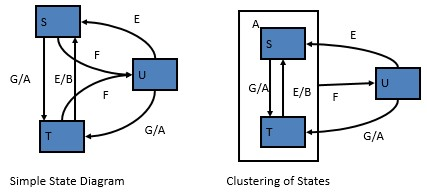
\includegraphics[width=12cm,height=5cm]{Screenshot.jpg}
\caption{Clustering}
\end{figure}
Clustering reduces number of transitions in a statechart Expanding state A showing its substates is called as refinement.\\


\subsection{Orthogonality}
In the above section we have seen that the state comprises of two or more states is a superstate. Examples in the above section, the superstate is the OR decomposition of states. In this section we introduce AND decomposition, capturing the property that, being in a state, the system must be in all of its AND components. The notation used in statecharts is the physical splitting of a box into components using dashed lines.\\
\noindent
\textbf{EXAMPLE:}\\
Figure3 shows a state C consisting of AND components A and B, with the property that being in C entails being in some combination of X,Y or Z with R or S. We say that C is the orthogonal product of A and B. The components A and B are no different conceptually from any other superstate; they have defaults, internal transitions,etc. Entering C from outside, in the absence of any additional information, is actually entering the combination (X, R) by the default arrow.If event t1 occurs, it transfers X to X itself and R to S, resulting in new combine state (X, S). This illustrates a certain kind of synchronization: a single event causing two simultaneous  happenings.\\
\begin{figure}[H]
\centering
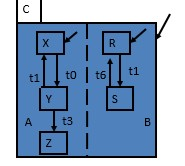
\includegraphics[width=7cm,height=5cm]{Screenshot002.jpg}
\caption{Orthogonality}
\end{figure}
\newpage
\subsection{Condition and Selection Entrances}
\textbf{Condition:}\\
Upon the entrance of the superstate a condition is checked and the transition is made to one of the sub-states in the superstate.\\ 
\begin{figure}[H]
\centering
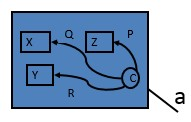
\includegraphics[width=7cm,height=5cm]{Screenshot004.jpg}
\caption{Conditional Entrance}
\end{figure}
\noindent
\textbf{Selection Entrance:}\\
The transition is made depending on the generic value of the input rather than the condition.
\begin{figure}[H]
\centering
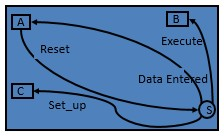
\includegraphics[width=7cm,height=5cm]{Screenshot005.jpg}
\caption{Selection Entrance:}
\end{figure}
\newpage
\subsection{Delays and Timeouts:}
Sometimes the transition from one state to another occurs precisely when the specified number of time units have elapsed from the occurence of the specified event.\\
\noindent
\textbf{EXAMPLE:}\\

\begin{figure}[H]
\centering
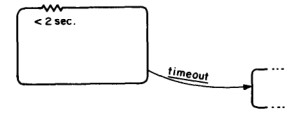
\includegraphics[width=7cm,height=5cm]{timeout.jpg}
\caption{Transition on Timeout}
\end{figure}
\subsection{Significance of System's History}
In a multi-superstate system when an event causes transition from one superstate to another, on what basis system will decide the transition to a particular substate of that superstate? Here is the answer. One of the most interesting  and frequent  ways of entering  a group of states is by the system\textquotesingle s history in that group. The simplest  kind of this enter-by-history  is entering  the state most recently  visited. Shallow history(H) represents the most recently entered state at the same level. Deep history represents entering the most recently visited state irrespective of how deep the state is. In the following example history chooses between G and F. H remembers between A, B, C, D, E. H remembers the last sub-state the system left. $H^*$-System will enter the most recently visited states. $H^*$ remembers the last sub-state the system left, irrespective of how deep it may be when considered with the history state. B and C are the default initial states for G and F.
\begin{figure}[H]
\centering
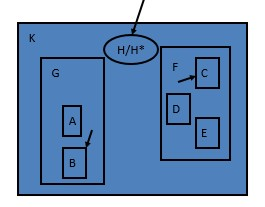
\includegraphics[width=8cm,height=6cm]{Screenshot003.jpg}
\caption{System's History}
\end{figure}
\section{Statechart Editor Tools}
The free to use, open source toolkit Statechart Tools (SCT) provides an integrated modeling environment for the specification and development of reactive, event-driven systems based on the concept of statecharts. Many statechart tools are available in the market. These statechart tools contains features like editing, simulation and code generation. The dynamic behaviour of system can be analyse using simulation feature. The code generation feature of statechart tools reduces development time.
\subsection{YAKINDU SCT Software}
This software gives all the features mentioned above. This software is easy to install and all the manuals are available at \href{https://www.itemis.com/en/yakindu/statechart-tools/}{YAKINDU SCT}.\\
This is a typical workspace of YAKINDU SCT.
\newpage
\begin{figure}[H]
\centering
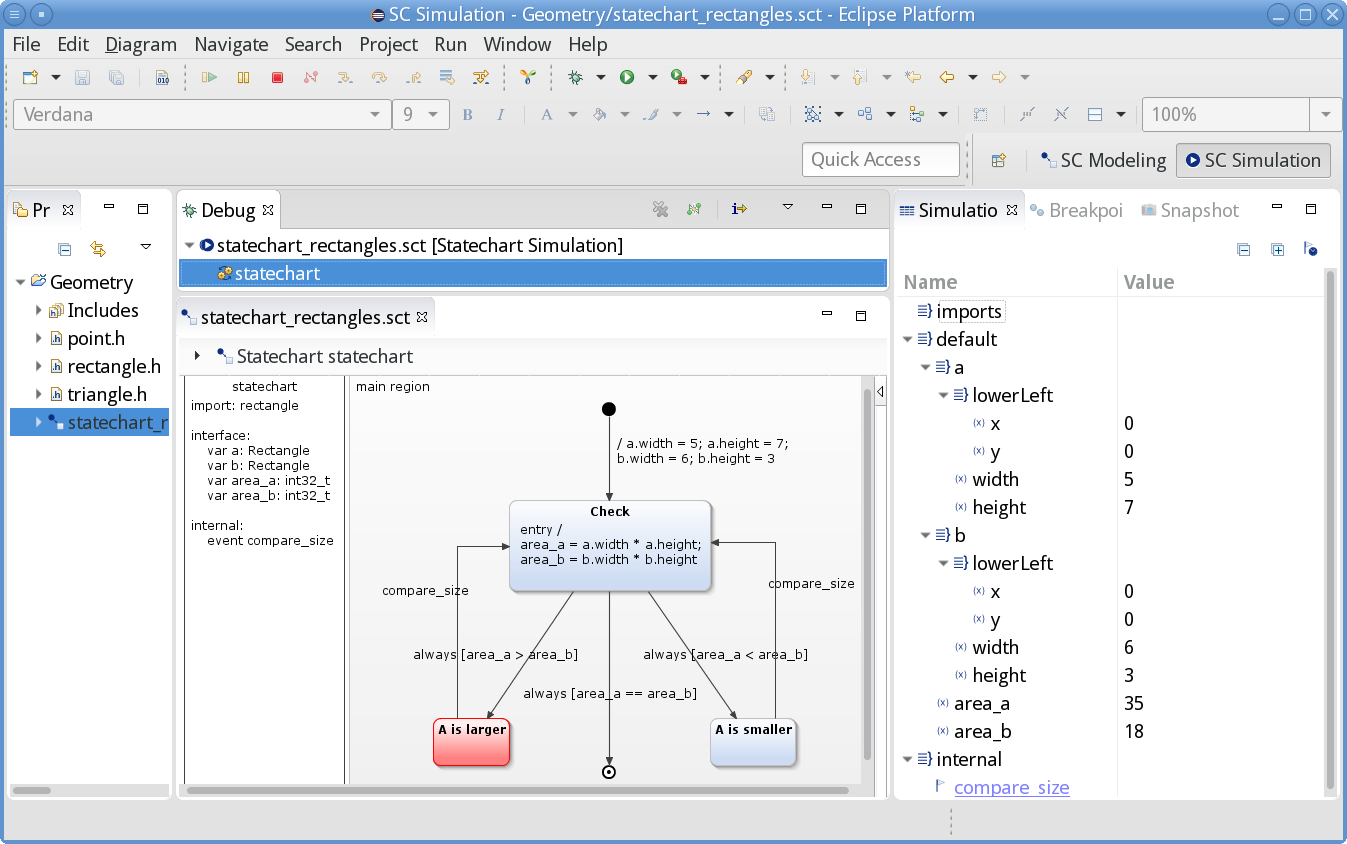
\includegraphics[width=14cm,height=10cm]{gui.png}
\caption{YAKINDU GUI}
\end{figure}
\newpage
\subsection{Features of YAKINDU SCT}
\begin{itemize}
\item Editing feature gives an intuitive combination of graphical and textual notation. While states, transitions and state hierarchies are graphical elements, all declarations and actions are specified using a textual notation.\\
\item The validation of state machines includes syntax and semantic checks of the full model.\\
\item The simulation of state machine models allows the dynamic semantics to be checked. Active states are directly highlighted in the statechart editor and a dedicated simulation perspective features access to execution controls, inspection and setting variables, as well as raising events.\\
\item The most important feature of YAKINDU SCT is code generation. SCT includes code generation for JAVA,C and CPP. Following image shows the code generation feature in YAKINDU SCT\\
\begin{figure}[H]
\centering
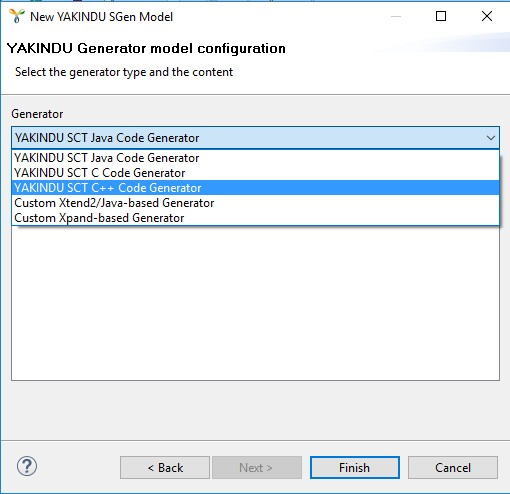
\includegraphics[width=14cm,height=13cm]{code.jpg}
\caption{Code Generation in YAKINU SCT}
\end{figure}
\end{itemize}
\newpage
\subsection{Tasks Modeled}
\subsubsection{Water Level Controller}
    This is a simple example of water level controller. This system first checks the water level in the tank. If tank is empty then it turns on the motor pump and increment he water level in statechart model when we simulate the model. When water level reaches to peak point it turns off the motor pump.\\
    \begin{figure}[H]
\centering
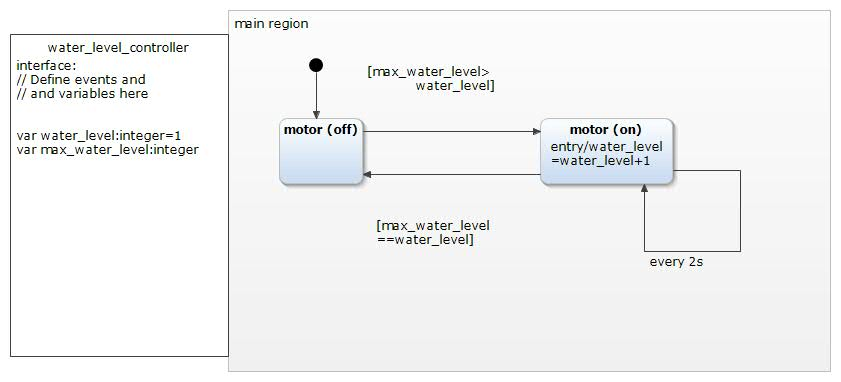
\includegraphics[width=15cm,height=6cm]{water_pump.jpg}
\caption{Water Level Controller}
\end{figure}
\newpage
\subsubsection{Real Time Clock}
This statechart model of real time clock converts time into a single integer value. Using few mathematical syntax we are converting this integer into hours, minutes and seconds to display. We can even set a particular time by generating SET event.\\
\begin{figure}[H]
\centering
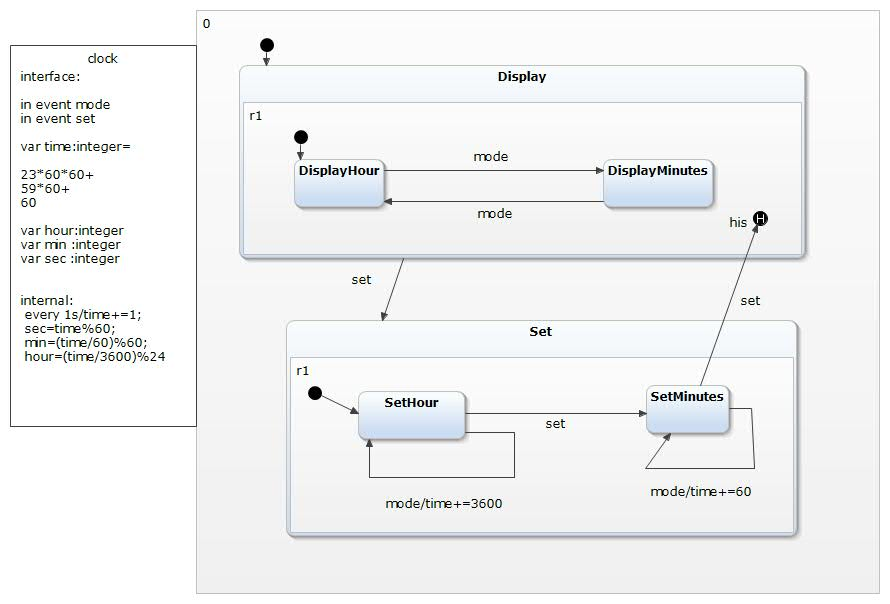
\includegraphics[width=12cm,height=9cm]{clock1.jpg}
\caption{Real Time Clock}
\end{figure}
\newpage

\subsubsection{Elevator System}
Following elevator model demonstrates the actual behaviour of an elevator system. When user enters floor number elevator door will get close and it will moves up till counter of floor number reaches to entered floor number. Once it reaches to the the destination; door will get open.

\begin{figure}[H]
\centering
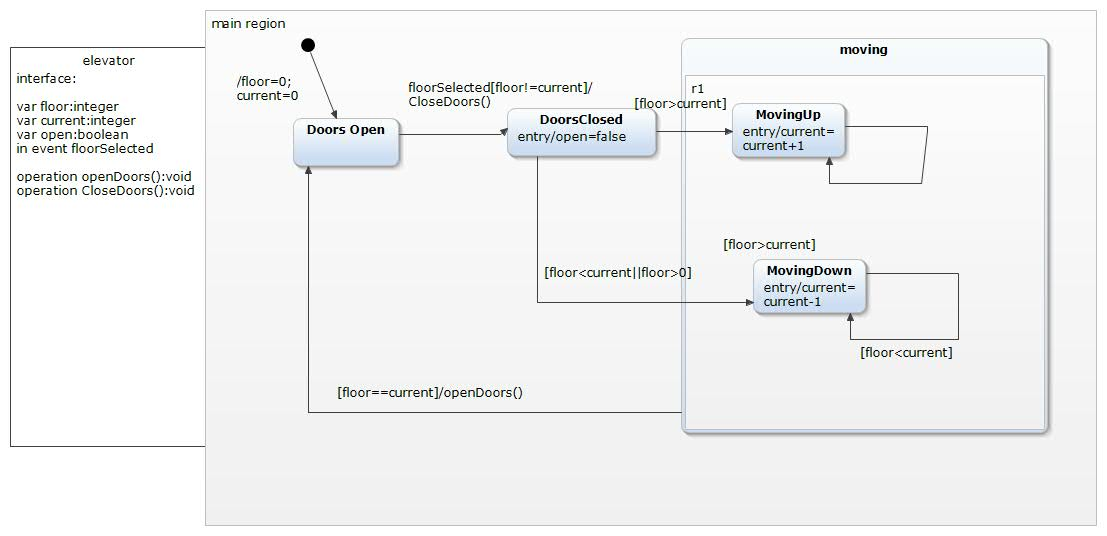
\includegraphics[width=15cm,height=12cm]{elevator.jpg}
\caption{Elevator System}
\end{figure}

\newpage
\subsection{Structure of C Code Generated by YAKINDU SCT }
\begin{itemize}
\item C code generator in YAKINDU Statechart Tool generates three header files. The {sc\_types.h} header file contains some basic definitions for C++ compiler compatibility and typedefs to map the YAKINDU statechart types to C types. The next header file is named after the statechart. Within this header file an enum containing the state names is defined as well as data structures for each of the statechart’s interfaces. Additionally a structure for the statechart’s time events is defined. If a statechart uses timing functionality or external operations, an additional header file is generated. Its name follows {statechart\_nameRequired.h} this pattern.
\item If we observe this header files and C code we can conclude that this is structured C code which is not Firebird V compatible or any other micro-controller.
\item The generated code contains fundamental methods to initialize, enter, and exit a state machine, as well as a method to start a run-to-completion step. So we could have thought of this structure
\begin{figure}[H]
\centering
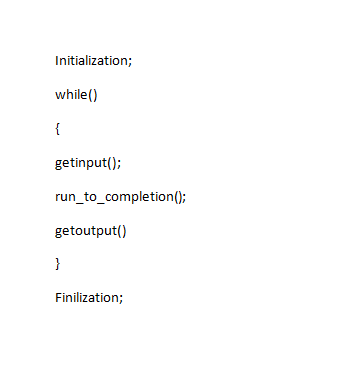
\includegraphics[width=8cm,height=6cm]{khuspe.PNG}
\caption{Structure of Code}
\end{figure}
\end{itemize}
\newpage
\subsection{Some High Level Models}

\subsubsection{Autonomous Shopping Robot} 

User has to order his/her products from the website. This order will get store in database. Arduino ethernet shield will extract the whole order, it will convert it in an appropriate packets and will send to Firebird V robot via bluetooth module. Robot will move around the shop to collect the products. Once all the products are collected by the robot it will send an acknowledgement to arduino and arduino will send a message to user via GSM module. For more details refer this \href{https://youtu.be/47TJFqiCook}{video}. 
\begin{figure}[H]
\centering
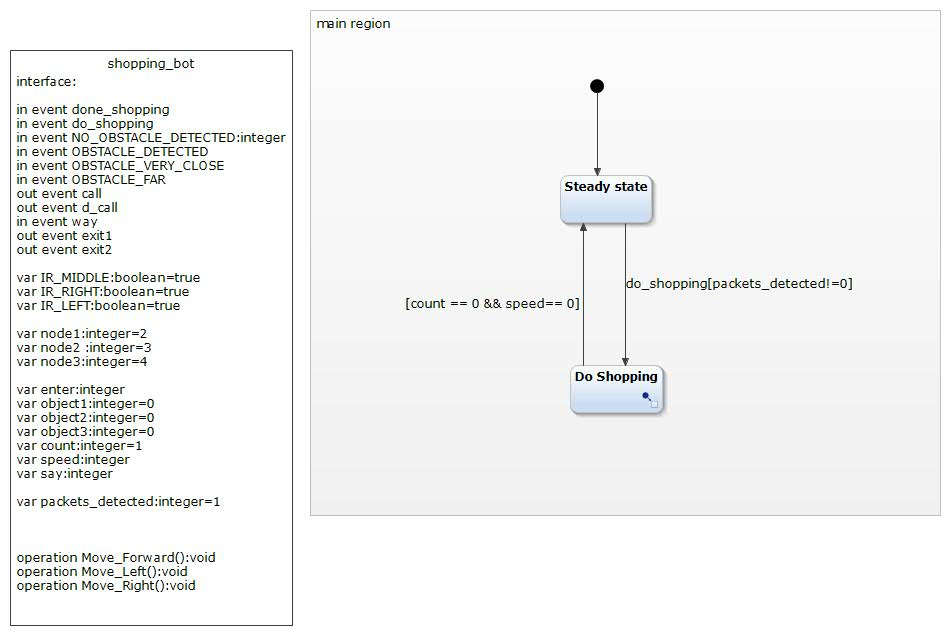
\includegraphics[width=16cm,height=10cm]{7.jpg}
\caption{Main Region}
\end{figure}
This State Machine diagram for Autonomous Shopping Robot gives the high level control flow of the Autonomous Shopping Robot function. Initially the system will be in \emph{steady} state, as no packages has been detected. The transition will take place from \emph{steady} state to do shopping state as soon as do shopping event has been raised. When  all the object has been collected then the transition takes place from \emph{do shopping} to \emph{steady} state as the work has been completed. In this statechart \emph{Do Shopping} state is a superstate which consists of two orthogonal states.\\
\begin{enumerate}
\item \textbf{White Line Follower and ACC} 
\begin{figure}[H]
\centering
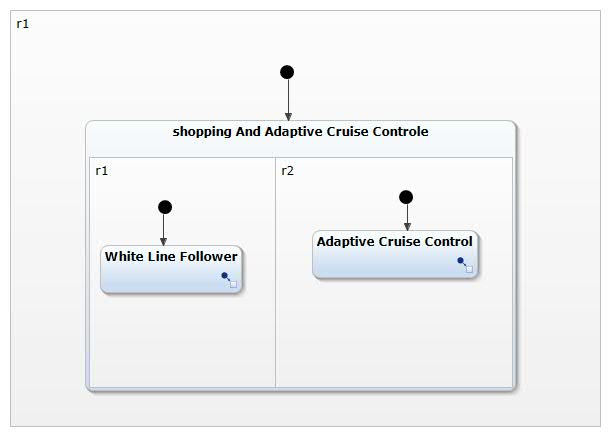
\includegraphics[width=10cm,height=9cm]{1.jpg}
\caption{White Line Follower and ACC}
\end{figure}
This is an orthogonal state which is inside the \emph{do shopping} state, in  orthogonal state two or more actions can be performed simultaneously.In the above diagram the orthogonal state has two substates. One substate is \emph{White line follower} and other one is \emph{adaptive cruise control}. The \emph{White Line follower} module carries out the activities needed to keep the robot moving a long the specified path. The \emph{Adaptive Cruise Control} module senses for obstacles on the path and avoids accident. Both are superstates too.\\
\item \textbf{White Line Follower}\\

This module is used to make the robot following the white line path laid out before it. The three white line sensors which are three inputs for this module. The left, middle and right sensors are referred by wsl, wsm and wsr respectively. The robot starts by being placed on the white line and moves forward. Using the sensor values we are continuously checking to see if it has veered off its path. Apart from this this module is keeping a track whether a node has been detected or not. If all the white line sensors are on white line then module detects the node and performs required tasks i.e. it increments the count on detection of each node and if that node matches with the node which has been entered by user, robot will stop at that node and collect the total amount of products entered by user.\\
\begin{figure}[H]
\centering
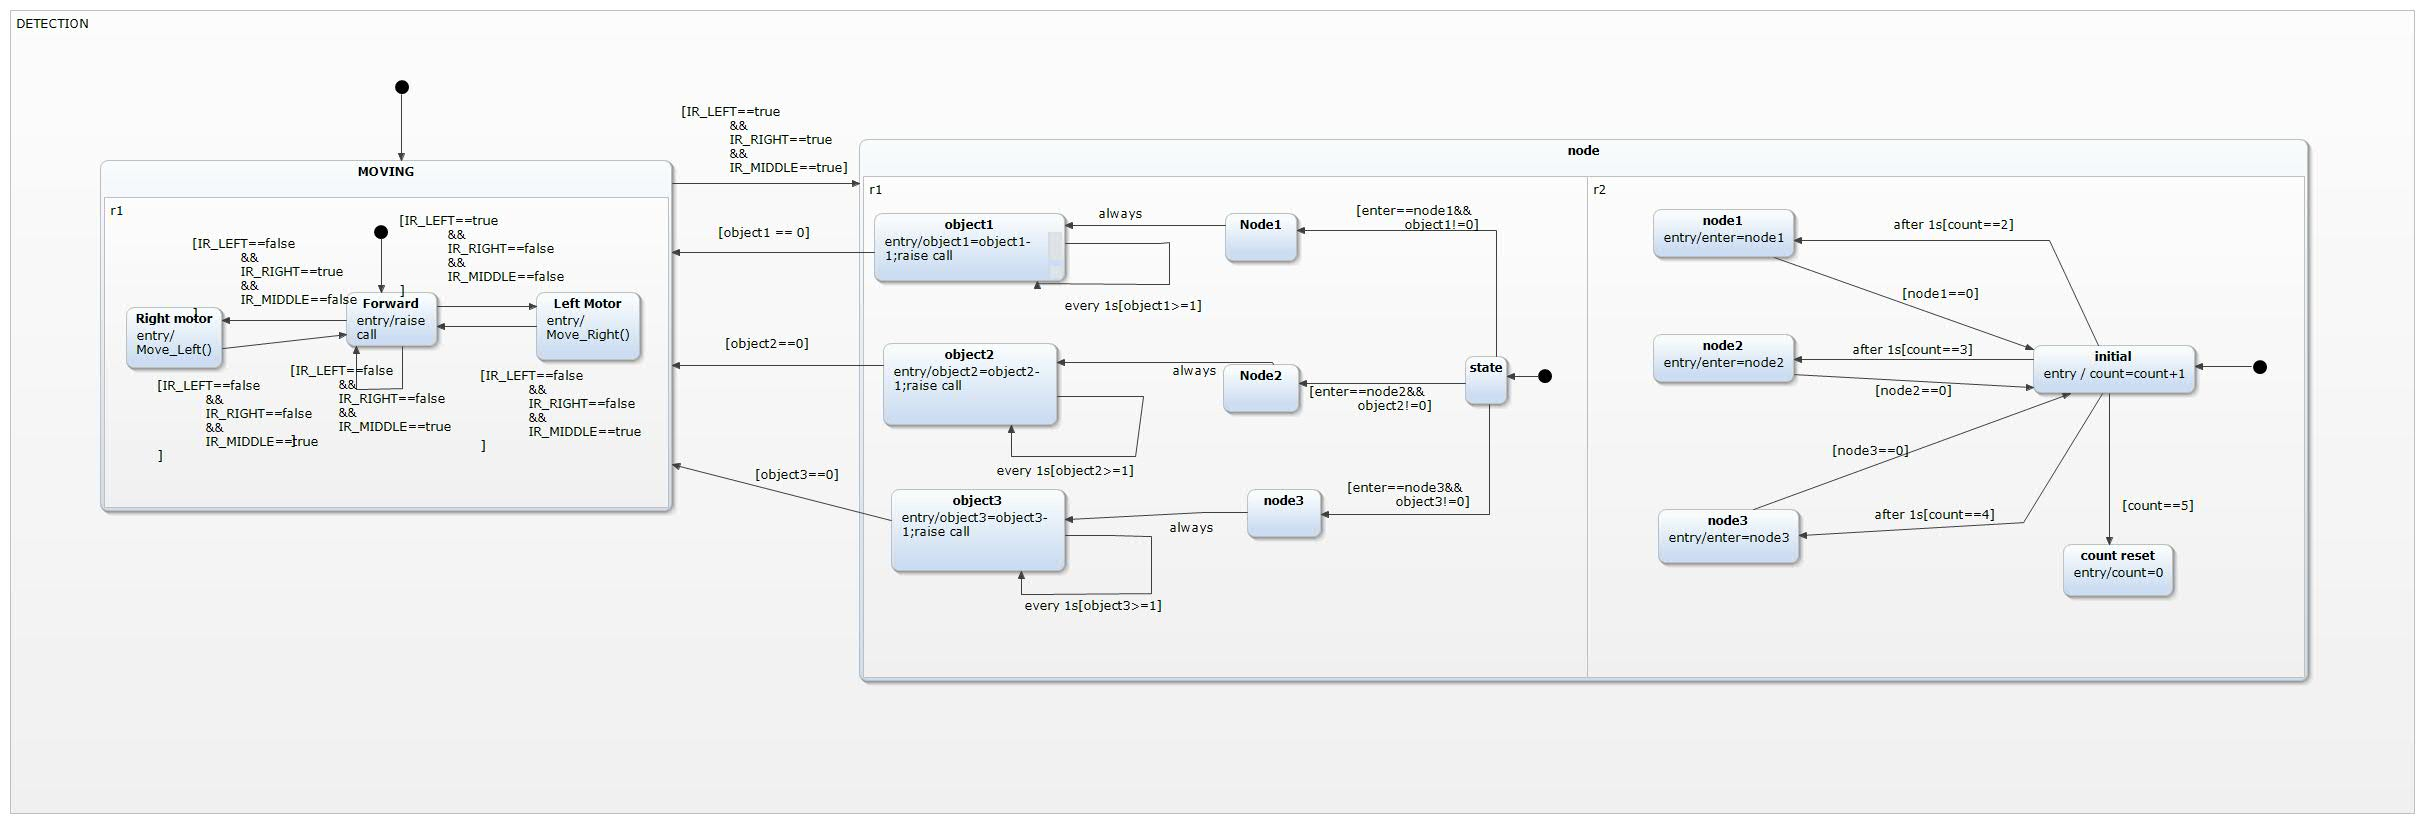
\includegraphics[width=25cm,height=16cm,angle=90]{44.jpg}
\caption{White Line Follower}
\end{figure}
\newpage
\item \textbf{Moving}\\
\begin{figure}[H]
\centering
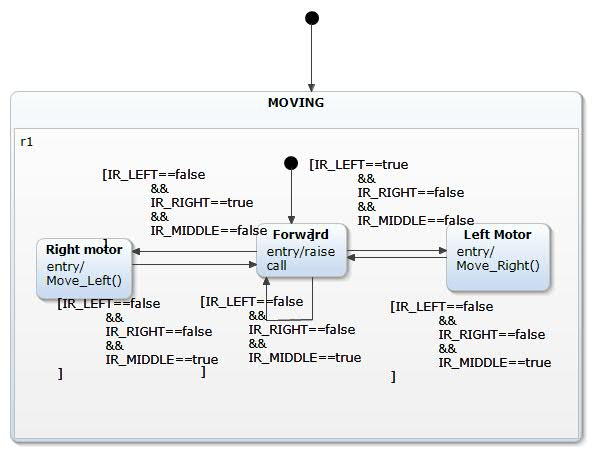
\includegraphics[width=13cm,height=12cm]{6.jpg}
\caption{Selection Entrance}
\end{figure}

 \begin{itemize}
 \item IR-LEFT\\
 This is an input from left hand side white line sensor. This is a boolean variable which gives true value on detection of white line.
 \item IR-RIGHT\\
  This is an input from right hand side white line sensor. This is a boolean variable which gives true value on detection of white line.
 \item IR-MIDDLE\\
  This is an input from middle white line sensor. This is a boolean variable which gives true value on detection of white line.\\
  A combination of all the three variables in the form of conditions makes a transition from one state to another state to drive the robot accordingly.
 \end{itemize}
 
 
\item \textbf{Node Detection}\\
\begin{figure}[H]
\centering
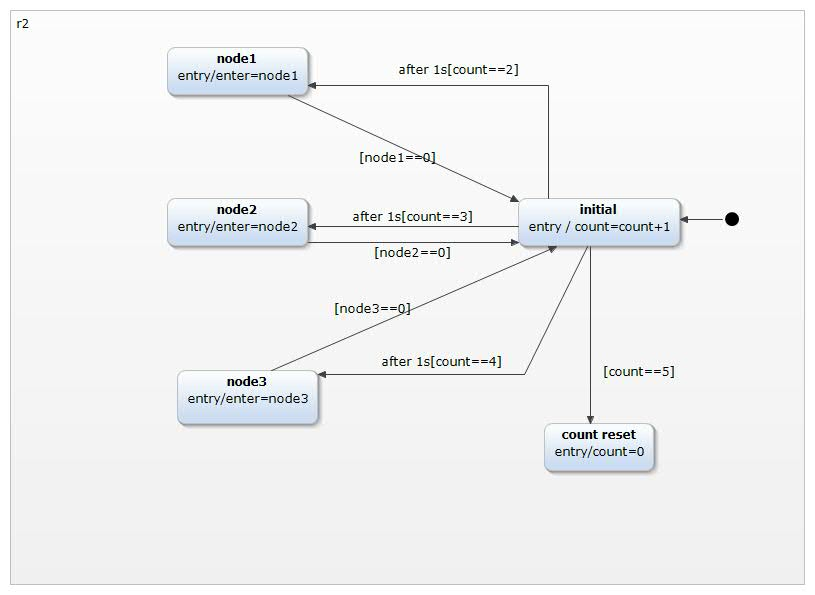
\includegraphics[width=15cm,height=12cm]{5.jpg}
\caption{Node Detection}
\end{figure}
This is a \emph{r2} region of state \emph{node}. When all the white line sensors gives true value transition will takes place to this state. In this state it will increment the counter by one on every detection of node. Then it will check whether this node is being entered by use or not. For this node1, node2 and node3 variables are being used by this state.
Since we are considering only three nodes, when a count value reaches to 5 it will reset it. On every detection of node enter variable will store the node value and this value is being used in the \emph{r1} region of state \emph{node}.\\
\newpage

\item \textbf{Node Detection}\\
\begin{figure}[H]
\centering
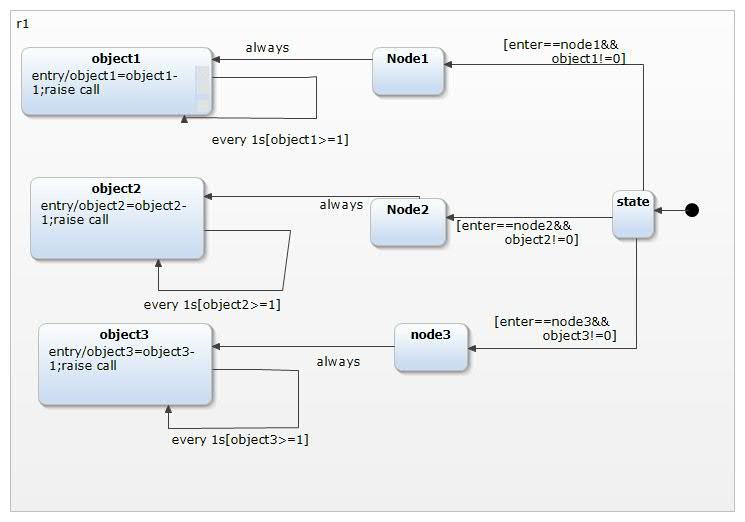
\includegraphics[width=17cm,height=13cm]{47.jpg}
\caption{Node Detection}
\end{figure}

This is a \emph{r1} region of \emph{node} state. Variables object1, object2 and object3 indicates the total number objects selected by user for each node. If user entered node matches with the value in enter variable and non zero value of variable object for each node then transition will takes place from by default state of region \emph{r1} to the respective \emph{object} state which decrements the value of object variable i.e. robot is collecting the products. When this value reaches to zero transition will takes place to the white line follower state. \\
\newpage

\item \textbf{Adaptive Cruise Control}\\
\begin{figure}[H]
\centering
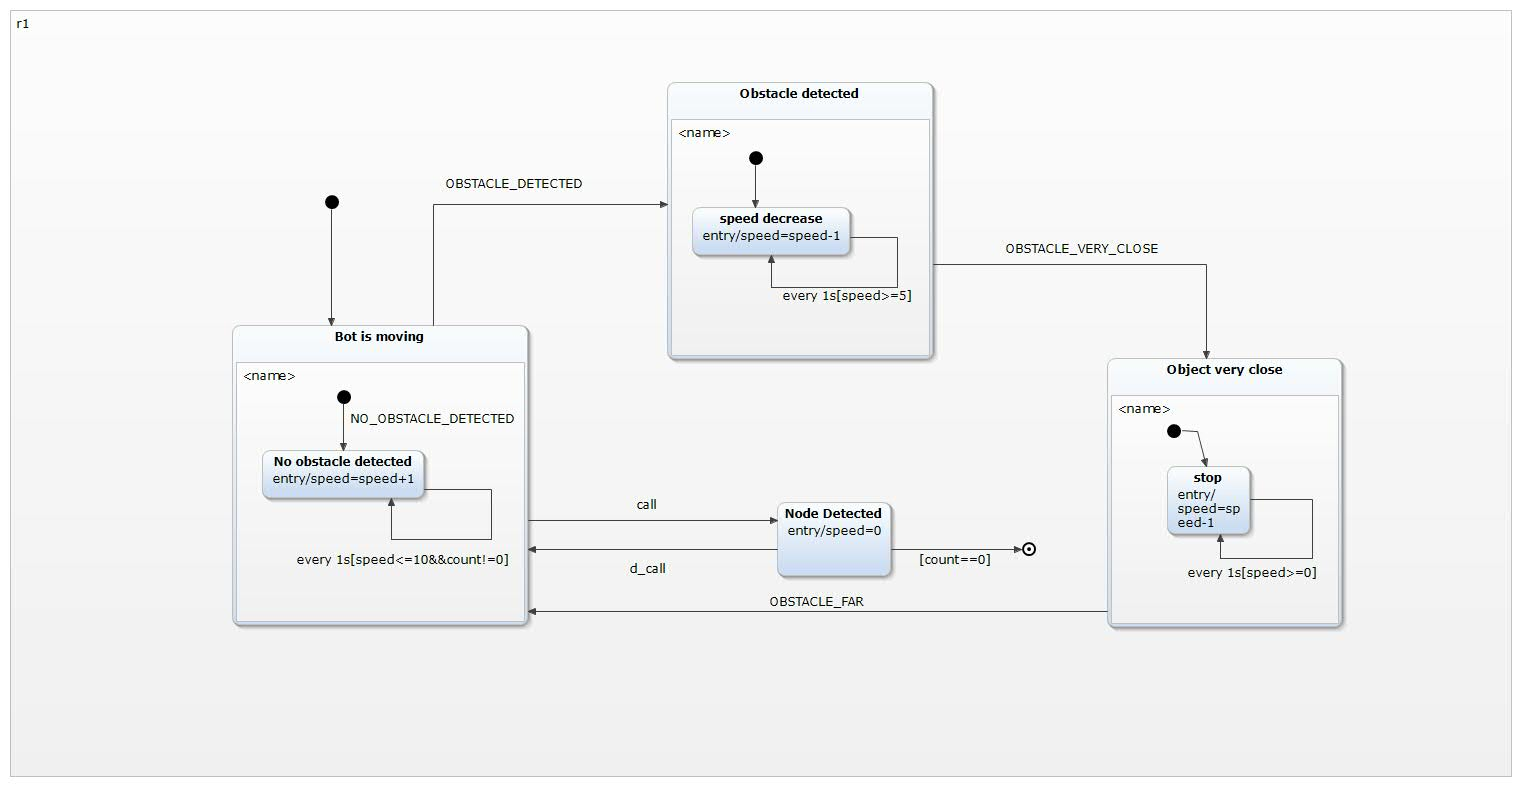
\includegraphics[width=16cm,height=13cm,angle=90]{4.jpg}
\caption{Adaptive Cruise Control}
\end{figure}
\newpage
This module ensures that robot does not hit any obstacle in its path. It takes its input from the front IR sensor and the front proximity sensor indicated by \textit{sharpc} and \textit{proxc} respectively. While the robot is moving, this module is continuously checking to see if there are any obstacles on the path. Depending on the distance of the obstacle, it performance certain actions. In this state default state is Bot is Moving. As long as robot is in state speed will keep on increasing. Depending on the distance of an obstacle from the robot, {OBSTACLE\_DETECTED}, {OBSTACLE\_FAR}, {OBSTACLE\_VERY\_CLOSE} events will get generate. When robot detects the required node an event call from \emph{White Line Follower} state will make transition from event Bot is Moving to Node Detected. And in the end if {node\_coun}t is zero robot will come out of this state.\\
\end{enumerate}
\subsubsection{Hazardous Waste Disposal}

In this theme, we have attempted to automate a system to transport Hazardous Waste and to place the waste in designated locations. The arena for this theme represents two areas: one City Area (CA) where the waste is generated and another Isolated Area (IA) where the waste has to be disposed. A water body separates CA and IA, which are connected by a bridge over the water. Different types of Hazardous Wastes are placed in random order stacked in CA. The robot should transfer these wastes to IA travelling across the bridge.\\
To know more about technicalities of this project one can see this \href{https://www.youtube.com/watch?v=L6Ta_fylXQA
}{video} or can refer the pdf describing the whole task which is available on github in hazardous waste disposal model.\\

\begin{itemize}
\item Following model is the main region of the model consists of four regions which runs parallel.
\item \emph{Task} region of this state first check for the status of the bridge. If bridge path is available then robot will pick the object and reach to junction state and then come back to initial state.\\
\item Once robot is reached to the junction it will check for the required node to drop the object.\\
\item \emph{Object status} region gives an information about an object robot is working. \\
\item To do this whole task robot will be using white line sensors. Region \emph{motion status} gives an information whether the robot is moving or not.\\
\end{itemize}
\newpage
\begin{figure}[H]
\centering
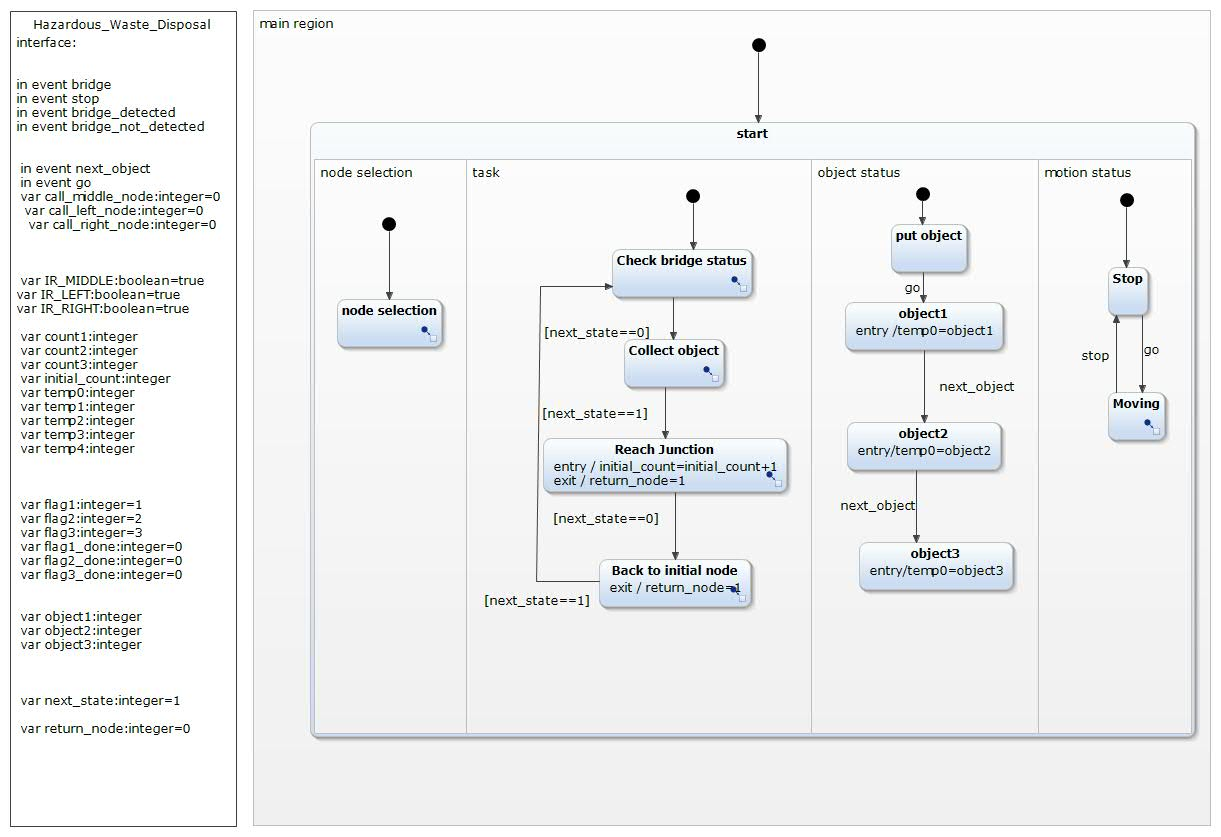
\includegraphics[width=18cm,height=14cm]{51.jpg}
\caption{Hazardous Waste Disposal}
\end{figure}
\newpage
\begin{enumerate}
\item \textbf{Check bridge status}\\
\begin{figure}[H]
\centering
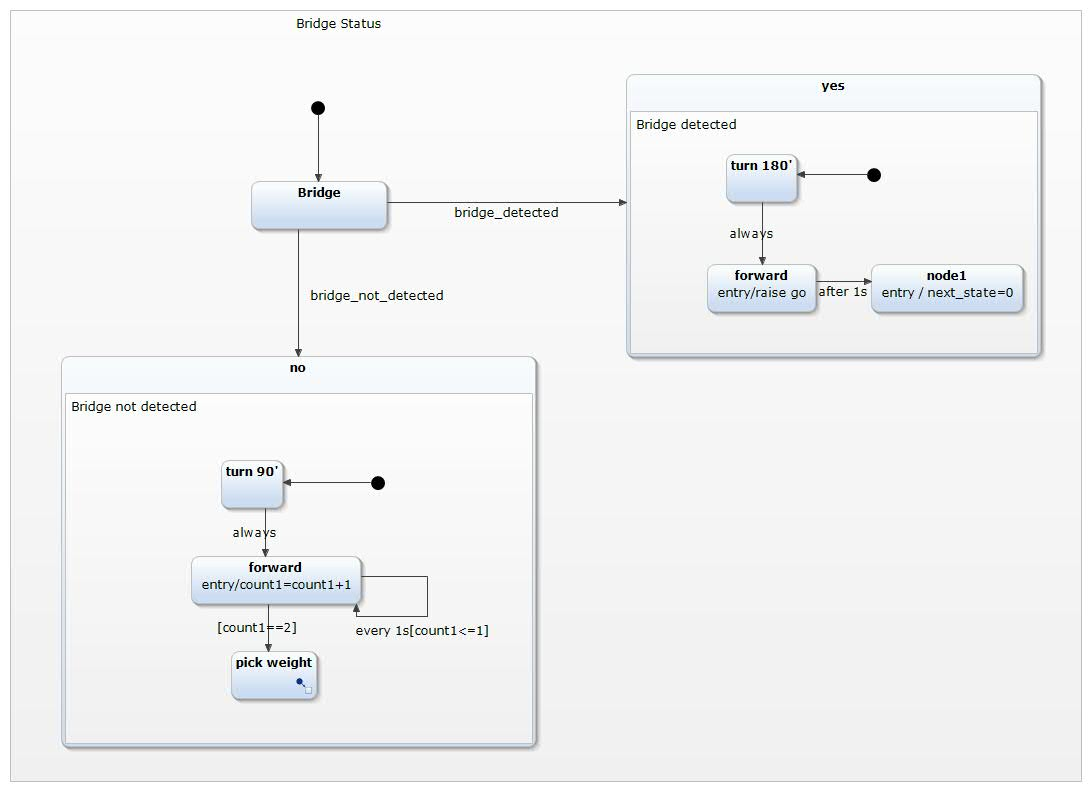
\includegraphics[width=16cm,height=11cm]{53.jpg}
\caption{Check Bridge Status}
\end{figure}
This states takes an input from front sharp sensor. If it detects bridge it means bridge is inclined towards robot side, means bridge path is free for robot. If it does not detect the bridge it means bridge is not inclined towards robot. This time an event {bridge\_not\_detected} makes transition from \emph{Bridge} to \emph{bridge not detected}. In this state  it will first pick up the weights and will drop in the tray for lowering the bridge.
\newpage
\item \textbf{Collect Object}\\
\begin{figure}[H]
\centering
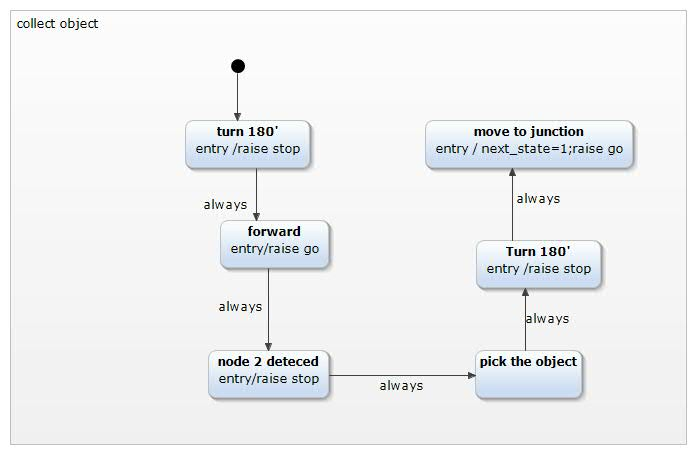
\includegraphics[width=14cm,height=9cm]{54.jpg}
\caption{Collect object}
\end{figure}
When bridge detected state creates a condition {node\_state$=$0} transition will takes place from check bridge state to collect object state. In this state robot will pick the object and turns 180 degree and moves to the junction with raising condition {next\_state$=$1} and raises an event go.\\

\item \textbf{Reach Junction}\\

This state consist of four substates. \emph{Node selection} is a by default state. When robot is at junction point this state will help to robot to decide which node it has to access. According to the raised condition transition will takes place from \emph{node selection} state to \emph{middle node}, \emph{right node}, or \emph{left node}. When robot picks up an object it stores the colour value of that object in variable temp0. Initially when it reaches to junction point it traverse all the nodes to check whether picked object matches with the flag value or not. If it does, robot will place an object at that node and stores the value of remaining flags. Flag1, flag2 and flag3 stores the value of an object which are placed on other side of bridge. Second time when robot comes with second object it will directly go to the respective node because all the values of flags are stored. Variable {initial\_count} is used for traversing of robot initially through all the flags. Variables {flag1\_done}, {flag2\_done} and {flag3\_done} are being used to indicate that an object has been placed on right node or not. Following image shows this entire explanation. \\
\newpage
\begin{figure}[H]
\centering
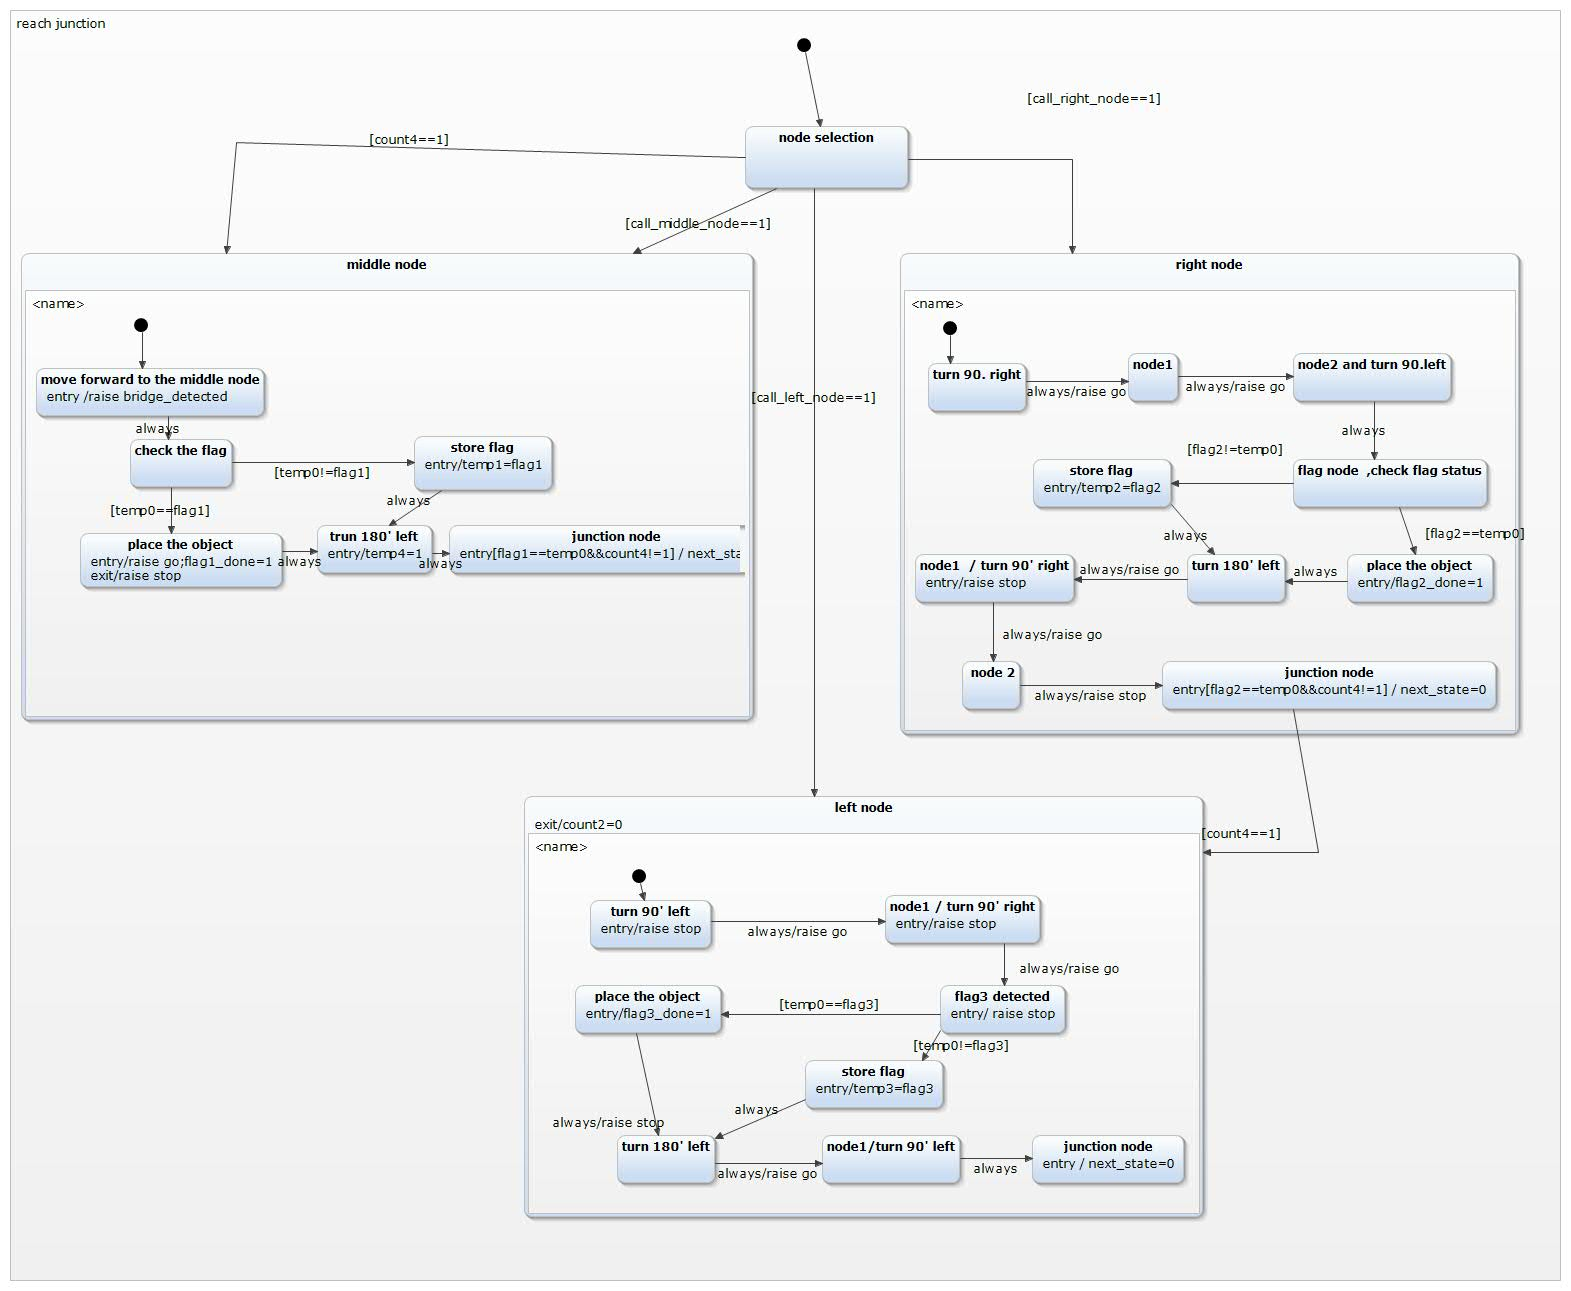
\includegraphics[width=20cm,height=18cm,angle=90]{55.jpg}
\caption{Reach Junction}
\end{figure}
\newpage

\item \textbf{Back to Initial Point}\\

After placing an object robot has to come back to its initial point to collect second object. For that it will first check for the bridge status and will function accordingly.

\begin{figure}[H]
\centering
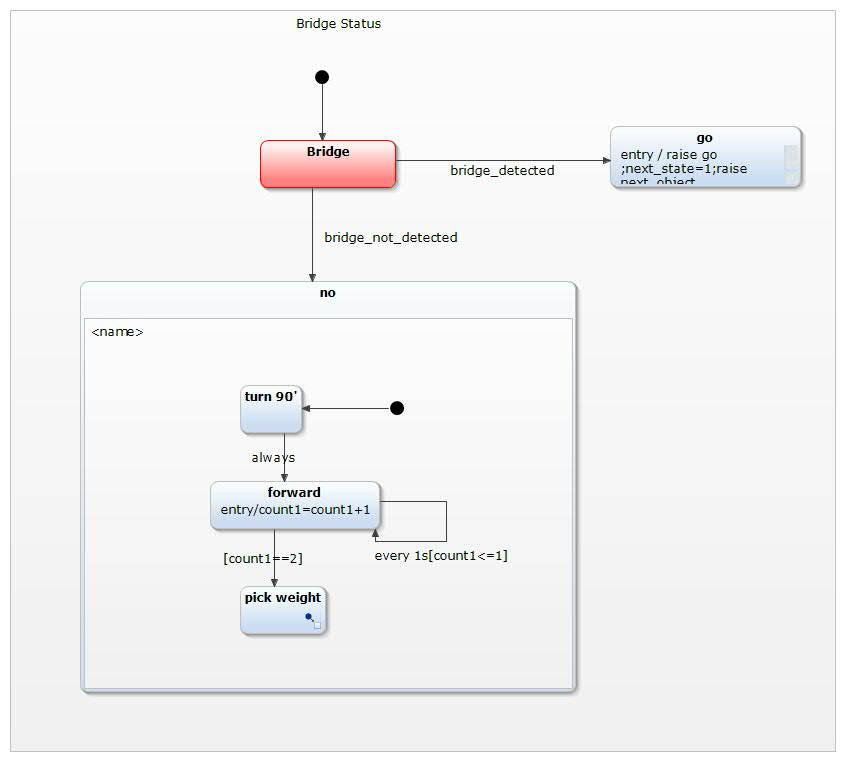
\includegraphics[width=14cm,height=10cm]{60.jpg}
\caption{Back to Initial Point}
\end{figure}

\item \textbf{Node Selection}\\

This state provides exact location of flag2 and flag3. After placing first object it generates {initial\_count$>$$=$1} condition for second and third object. For second and third object it will set {call\_middle\_node}, {call\_right\_node} or {call\_left\_node} variables for appropriate transitions.

\newpage
\begin{figure}[H]
\centering
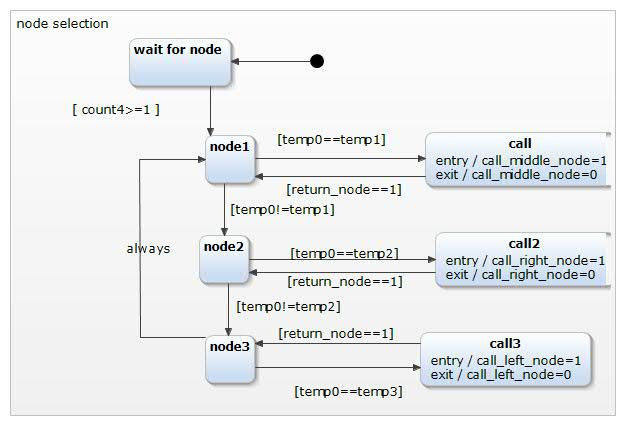
\includegraphics[width=12cm,height=9cm]{52.jpg}
\caption{Node Selection}
\end{figure}

\item \textbf{Object Status}\\

This state gives appropriate value to the temp0 variable when go event arises. When an event {next\_object} gets generated by Back to initial node state it will make a transition from object1 state to object2 state and so on. On every transition temp0 variable stores the value of object1, object2 or object3 variable. This variables are nothing but colour values of an object picked up by the robot.
\newpage
\begin{figure}[H]
\centering
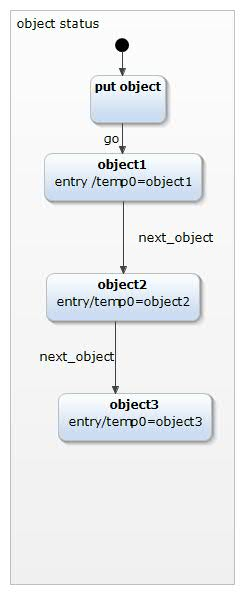
\includegraphics[width=7cm,height=12cm]{57.jpg}
\caption{Object Status}
\end{figure}

\item \textbf{Motion status}\\

This state describes the motion of robot. To perform whole task robot will be using white line follow sensors. When any state generates go event transition will takes place to Moving state. This Moving state consists of all the white line sensor variables.\\
\begin{itemize}
 \item IR-LEFT\\
 This is an input from left hand side white line sensor. This is a boolean variable which gives true value on detection of white line.
 \item IR-RIGHT\\
  This is an input from right hand side white line sensor. This is a boolean variable which gives true value on detection of white line.
 \item IR-MIDDLE\\
  This is an input from middle white line sensor. This is a boolean variable which gives true value on detection of white line.\\
  A combination of all the three variables in the form of conditions makes a transition from one state to another state to drive the robot accordingly.
\end{itemize}
\begin{figure}[H]
\centering
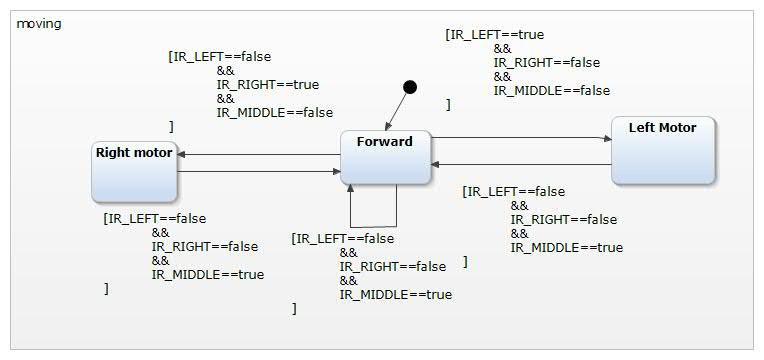
\includegraphics[width=16cm,height=12cm]{61.jpg}
\caption{Moving}
\end{figure}
\end{enumerate}
\newpage
\subsection{Difficulties Faced in Code Generation}
\begin{itemize}
\item Since we know that YAKINDU statechart tool can generate a code in C, CPP and JAVA. Firebird V contains ATmega2560, 8051 or LPC2148 microcontroller. This microcontroller needs embedded-C language for functioning.
\item C code generated by YAKINDU statechart tool is in structured C format. We had to convert it into embedded-C format in order to make it Firebird V compatible.
\item But we could not decode the code properly. So we decided to follow  \href{http://scholtyssek.org/blog/2013/10/21/yakindu-statechart-tools-arduino-integration/}{Marco's Blog}. He used the code generator feature of software in context of embedded systems and he decided to generate a code for Arduino UNO; therefore he modified statechart \emph{TrafficLight} example and implemented some simple glue code to map the hardware timer and the I/O-ports. We followed every step given in Marco\textquotesingle s blog but we failed to do it because he has not explained how and exactly where the glue code suppose to be added.
\item We tried to solve this problem using one more blog. This blog is Developing Software for Arduino with YAKINDU Statechart Tool. It enables you to develop software for the Arduino platform inside of Eclipse, instead of using the standard Arduino IDE.
\item In this blog he has generated  \emph{trafficlight} example code for  Arduino UNO. But how he has modified the code for Arduino is still unexplained.
\item By observing the  header files which are explained section and C file we can conclude that this generated code is in structured C format. Which is not Firebird V compatible. 
\item So we tried with another software which is Quantum Modeling. This software is used to generate the code for Arduino Platform. But it is quiet difficult to understand and model the tasks using QM tool.
\end{itemize}
\subsection{Glitches in YAKINDU Software}

In orthogonal state left hand side region can generate an event and right hand side can capture this event but vice versa is not possible means event generated by right hand side cant get captured by left hand side. This is a major problem we have faced. But we can convert this events into conditions for appropriate transition from one state to another state.\\


\subsection{Future Work}

In future one can try to understand this generated code in better way and can try to make it Firebird V compatible or with any other micro-controller. We can explore few more statechart tools like KSE and QM.

\subsection{Conclusion}

Since an ultimate goal of this project is to reduce the development time for building any system. And we can conclude that it is possible to do it with statechart modeling. But our observation says that available open source tools like YAKINDU are not yet developed to automatic generate the code which will be compatible with any micro-controller.\\


\begin{thebibliography}{5}
 \bibitem{1} David Harel, "Statecharts: A visual formalism for complex systems", \emph{Department of applied mathematics, The Weizmann Institute of Science, Rehovot, Israel}.
 \bibitem{2} Kavi Arya, Blossom Coelho, Shradda Pandya, "A Model Based Approach to System Building Using the E-Yantra Educatonal Robot", \emph{Department of Computer Science, IIT Bombay}.
 \bibitem{3} "Autonomous Robotic Parking Vehicle", \emph{Department of Computer Science, IIT Bombay}.
 \bibitem{3} Yakindu Statechart Tool \href{https://www.itemis.com/en/yakindu/statechart-tools/documentation/user-guide/}{Documentation}
 \bibitem{4} Yakindu Statechart Tool \href{https://www.itemis.com/en/yakindu/statechart-tools/documentation/tutorials/#oss_five-minutes-tutorial}{Tutorials}
 \bibitem{5} Quantum Modeling Tool \href{http://www.state-machine.com/qm/}{http://www.state-machine.com/qm/}
\end{thebibliography}


\end{document}

